\documentclass[11pt,a4paper]{article}

% Paquetes de idioma y codificación
\usepackage[utf8]{inputenc}
\usepackage[spanish,es-tabla]{babel}
\usepackage[T1]{fontenc}

% Tipografía moderna y microtipografía
\usepackage{lmodern}
\usepackage{microtype}

% Geometría de la página
\usepackage[margin=2.5cm]{geometry}

% Paquetes para matemáticas, gráficos y formato
\usepackage{amsmath}
\usepackage{amsfonts}
\usepackage{graphicx}
\usepackage{authblk}
\usepackage{titlesec}
\usepackage{setspace}
\usepackage{hyperref}
\usepackage{booktabs}
\usepackage{cite}

% Ajuste del formato de los títulos
\titleformat{\section}{\large\bfseries}{\thesection}{1em}{}
\titlespacing*{\section}{0pt}{1.2ex plus 1ex minus .2ex}{0.5ex plus .2ex}

% Información del documento
\title{\vspace{-2cm}\Large\bfseries Optimización Evolutiva y Multiobjetivo de Máquinas de Soporte Vectorial Cuántico con Ruido Realista para Física de Altas Energías}

\author[1]{Camilo A. Huertas-Archila}
\author[1]{Laura Isabel Nieto}
\author[1]{Carlos Andrés Gomez Vasco}
\affil[1]{\small Programa Académico de Física, Universidad Distrital Francisco José de Caldas, Bogotá, Colombia.}

\date{} 

\begin{document}

\maketitle
\thispagestyle{empty} 

\vspace{-1cm}
\begin{abstract}
\noindent
La discriminación de señales de partículas frente al ruido de fondo es un desafío central en la física de altas energías. Este trabajo explora la viabilidad de las Máquinas de Soporte Vectorial Cuántico (QSVM) para la clasificación de eventos cinemáticos del conjunto de datos SUSY, utilizando exclusivamente las características crudas de los detectores sin variables derivadas artificialmente. Se implementó una línea base clásica (SVM RBF) que alcanzó una precisión del $75.92\%$. Al evaluar enfoques cuánticos estándar, se demostró empíricamente la paradoja de la expresividad: mapas de características rígidos de alta dimensión (Fidelity Quantum Kernel) fallan al capturar correlaciones cinemáticas complejas, produciendo precisión aleatoria. La proyección de estados cuánticos en observables clásicos (Projected Quantum Kernel) mitigó parcialmente este problema, alcanzando un AUC de $0.847$. Sin embargo, las curvas de aprendizaje asintóticas demostraron que la topología rígida de los circuitos limita la generalización (estancamiento en $73\%$). Estos hallazgos sientan las bases empíricas para la futura implementación de un marco de optimización evolutiva multiobjetivo (GA-QSVM), diseñado para adaptar dinámicamente la arquitectura del circuito a las propiedades físicas del problema, minimizando la profundidad y la susceptibilidad al ruido en hardware NISQ.

\vspace{0.5cm}
\noindent \textbf{Palabras clave:} Computación Cuántica, Física de Altas Energías, QSVM, Aprendizaje Automático Cuántico, SUSY, Kernel Proyectado, Algoritmos Genéticos.
\end{abstract}

\vspace{0.5cm}

% ==========================================
% 1. INTRODUCCIÓN
% ==========================================
\section{Introducción}
El análisis de colisiones en aceleradores de partículas requiere separar eventos de señales extremadamente raras, como la producción de partículas supersimétricas (SUSY), de procesos de fondo dominantes regidos por el Modelo Estándar. Tradicionalmente, los físicos diseñan características cinemáticas de alto nivel derivadas de mediciones crudas para entrenar algoritmos de aprendizaje automático clásico \cite{baldi2014}. 

Recientemente, el Aprendizaje Automático Cuántico (QML) ha surgido como una alternativa prometedora. Las Máquinas de Soporte Vectorial Cuántico (QSVM) mapean datos clásicos a un espacio de Hilbert de alta dimensión mediante un \textit{ansatz} o circuito parametrizado, con el potencial de encontrar hiperplanos de separación inaccesibles para el cómputo clásico \cite{havlicek2019}. Sin embargo, los enfoques convencionales dependen de circuitos fijos que a menudo no logran generalizar adecuadamente a través de diferentes conjuntos de datos \cite{nguyen2026}. Un problema recurrente es que los circuitos altamente expresivos inducen una pérdida de varianza en la matriz del kernel (conocido como desvanecimiento del kernel), lo que impide el entrenamiento efectivo.

En este documento se analiza exhaustivamente el rendimiento de los QSVM con arquitecturas rígidas (estándar y proyectadas) aplicadas a la cinemática cruda del dataset SUSY, estableciendo el marco empírico que justifica la necesidad de evolucionar dinámicamente el diseño de los circuitos cuánticos.

% ==========================================
% 2. METODOLOGÍA
% ==========================================
\section{Metodología}

\subsection{Conjunto de Datos y Preprocesamiento}
Se utilizó el conjunto de datos SUSY de referencia \cite{baldi2014}. Para evaluar la capacidad intrínseca de los modelos, el espacio de características se redujo estrictamente a las primeras ocho variables ($n=8$), las cuales corresponden a mediciones cinemáticas puras de los detectores (momentos transversales, pseudorapideces, etc.). Las diez variables derivadas matemáticamente se excluyeron. Los datos fueron transformados mediante un escalador \textit{MinMax} al rango angular $[0, 2\pi]$ para ser codificados físicamente en las rotaciones de los qubits.

\subsection{Máquina de Soporte Vectorial Clásica (Línea Base)}
Se entrenó un modelo clásico utilizando un SVM con kernel de base radial (RBF). A través de una búsqueda de hiperparámetros con validación cruzada ($k$-Fold), se optimizaron el margen de regularización ($C$) y la dispersión del kernel ($\gamma$) para establecer el límite de precisión clásico esperado.

\subsection{Máquina de Soporte Vectorial Cuántico (QSVM)}
La formulación cuántica se basa en evaluar similitudes en el espacio de estados. Se evaluaron dos enfoques principales:

\textbf{1. Fidelity Quantum Kernel (FQK):} Mide la similitud global entre dos estados cuánticos codificados $|\psi(x_i)\rangle$ y $|\psi(x_j)\rangle$:
\begin{equation}
    K^{FQK}(x_i, x_j) = |\langle \psi(x_i) | \psi(x_j) \rangle|^2
\end{equation}

\textbf{2. Projected Quantum Kernel (PQK):} Para mitigar la maldición de la dimensionalidad, los estados se proyectaron a representaciones clásicas aproximadas evaluando la matriz de densidad reducida de una partícula (1-RDM) para cada qubit \cite{huang2021}:
\begin{equation}
    \rho_k(x_i) = \text{Tr}_{j \neq k}[\rho(x_i)]
\end{equation}
Las características cuánticas extraídas se pasaron a un kernel RBF clásico, permitiendo evaluar las expectativas de los operadores de Pauli ($X, Y, Z$).

% ==========================================
% 3. RESULTADOS Y DISCUSIÓN
% ==========================================
\section{Resultados y Discusión}

\subsection{Rendimiento Clásico (Línea de Referencia)}
La optimización del SVM clásico convergió hacia un margen rígido ($C=100, \gamma=0.01$), alcanzando una precisión general del $75.92\%$ y un Área Bajo la Curva (AUC) de $0.828$. Este resultado establece el umbral empírico a superar por los métodos cuánticos.

\subsection{Limitaciones del FQK y la Paradoja de la Expresividad}
La aplicación del FQK sobre las 8 características demostró un colapso en la generalización al aumentar la complejidad del \textit{ansatz}. El circuito simple sin entrelazamiento (\texttt{ZFeatureMap}) obtuvo $58.75\%$, superando a los mapas con entrelazamiento lineal (\texttt{ZZFeatureMap} y \texttt{PauliFeatureMap}), que decayeron a $53.75\%$. Esto confirma empíricamente que inyectar profundidad y entrelazamiento de manera rígida dispersa los estados en el espacio de Hilbert, disipando la estructura topológica de los datos cinemáticos.

\subsection{Rendimiento del Kernel Cuántico Proyectado (PQK)}
Al cambiar la formulación al PQK, la convergencia mejoró drásticamente. El modelo proyectado (\texttt{ZFeatureMap}, $reps=1$, $C=1$, $\gamma=0.01$) logró un AUC de $0.847$, superando la capacidad probabilística del modelo clásico (Figura 1).

\begin{figure}[h]
    \centering
    % Descomentar y ajustar la ruta de la imagen en Overleaf
     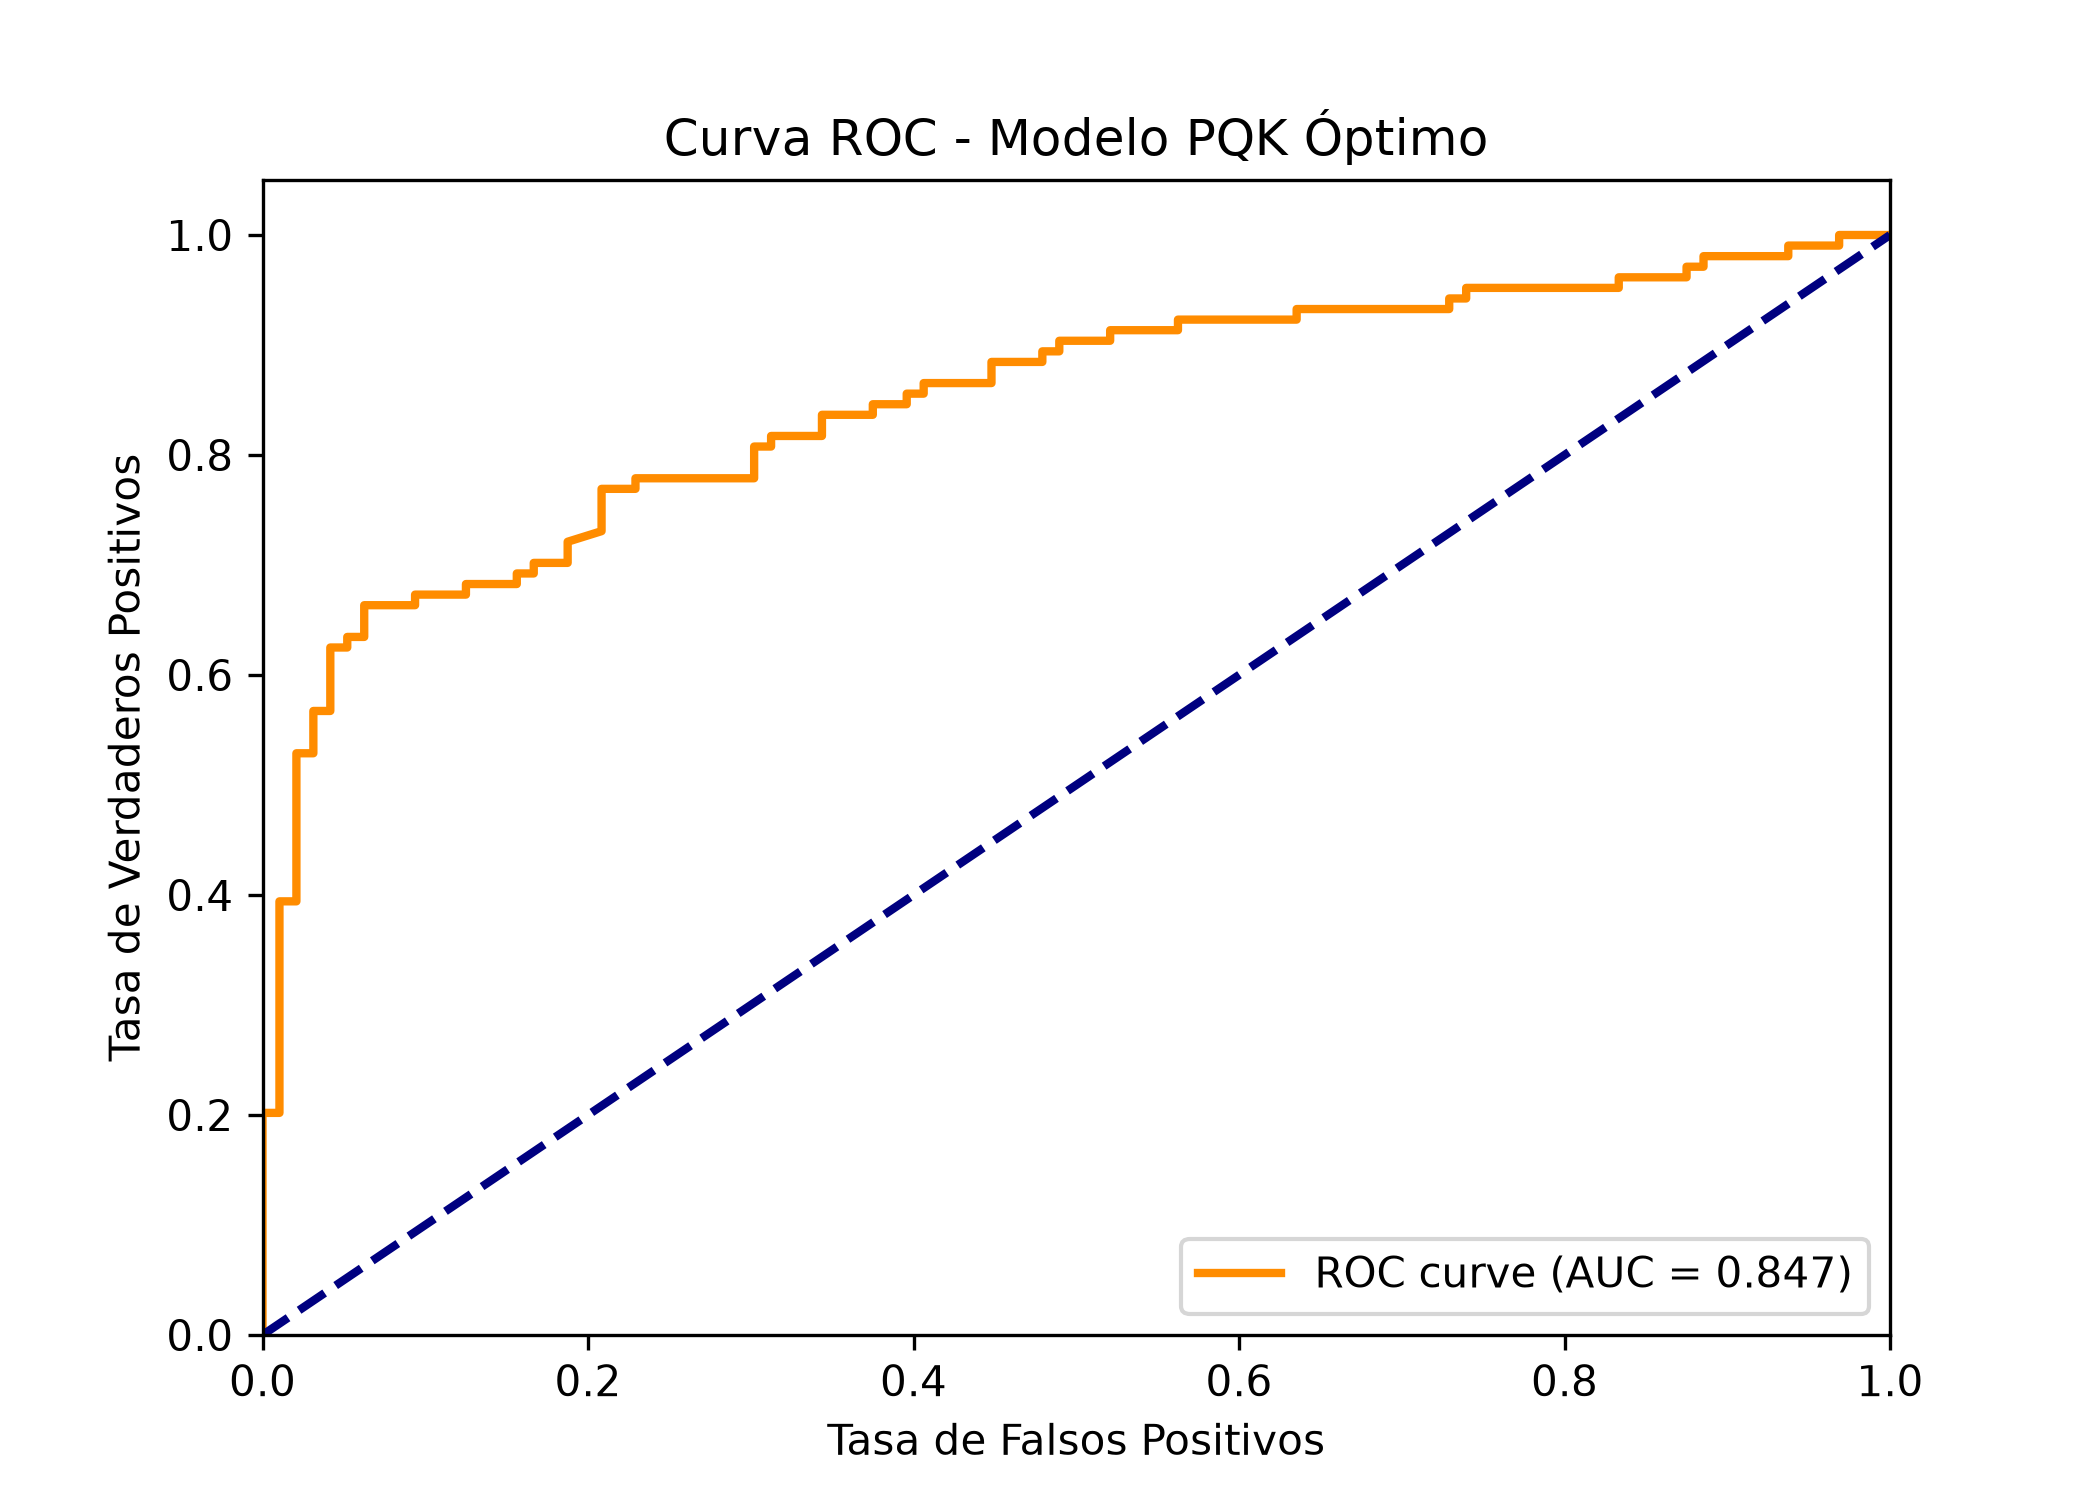
\includegraphics[width=0.6\textwidth]{curva_roc_pqk.png}
    \caption{Curva ROC y AUC para el modelo QSVM-PQK con profundidad reps=1.}
    \label{fig:roc}
\end{figure}

Sin embargo, el análisis de la matriz de confusión demostró que, aunque el circuito tiene una alta sensibilidad para clasificar el fondo del Modelo Estándar (verdaderos negativos), presenta deficiencias capturando la cinemática no lineal de la anomalía SUSY pura.

\subsection{Curva de Aprendizaje y Estancamiento Asintótico}
Para descartar la influencia del tamaño muestral, se analizó la precisión de validación cruzada ($k=5$) escalando el volumen de datos de 200 a 2000 eventos (Figura 2). 

\begin{figure}[h]
    \centering
    % Descomentar y ajustar la ruta de la imagen en Overleaf
     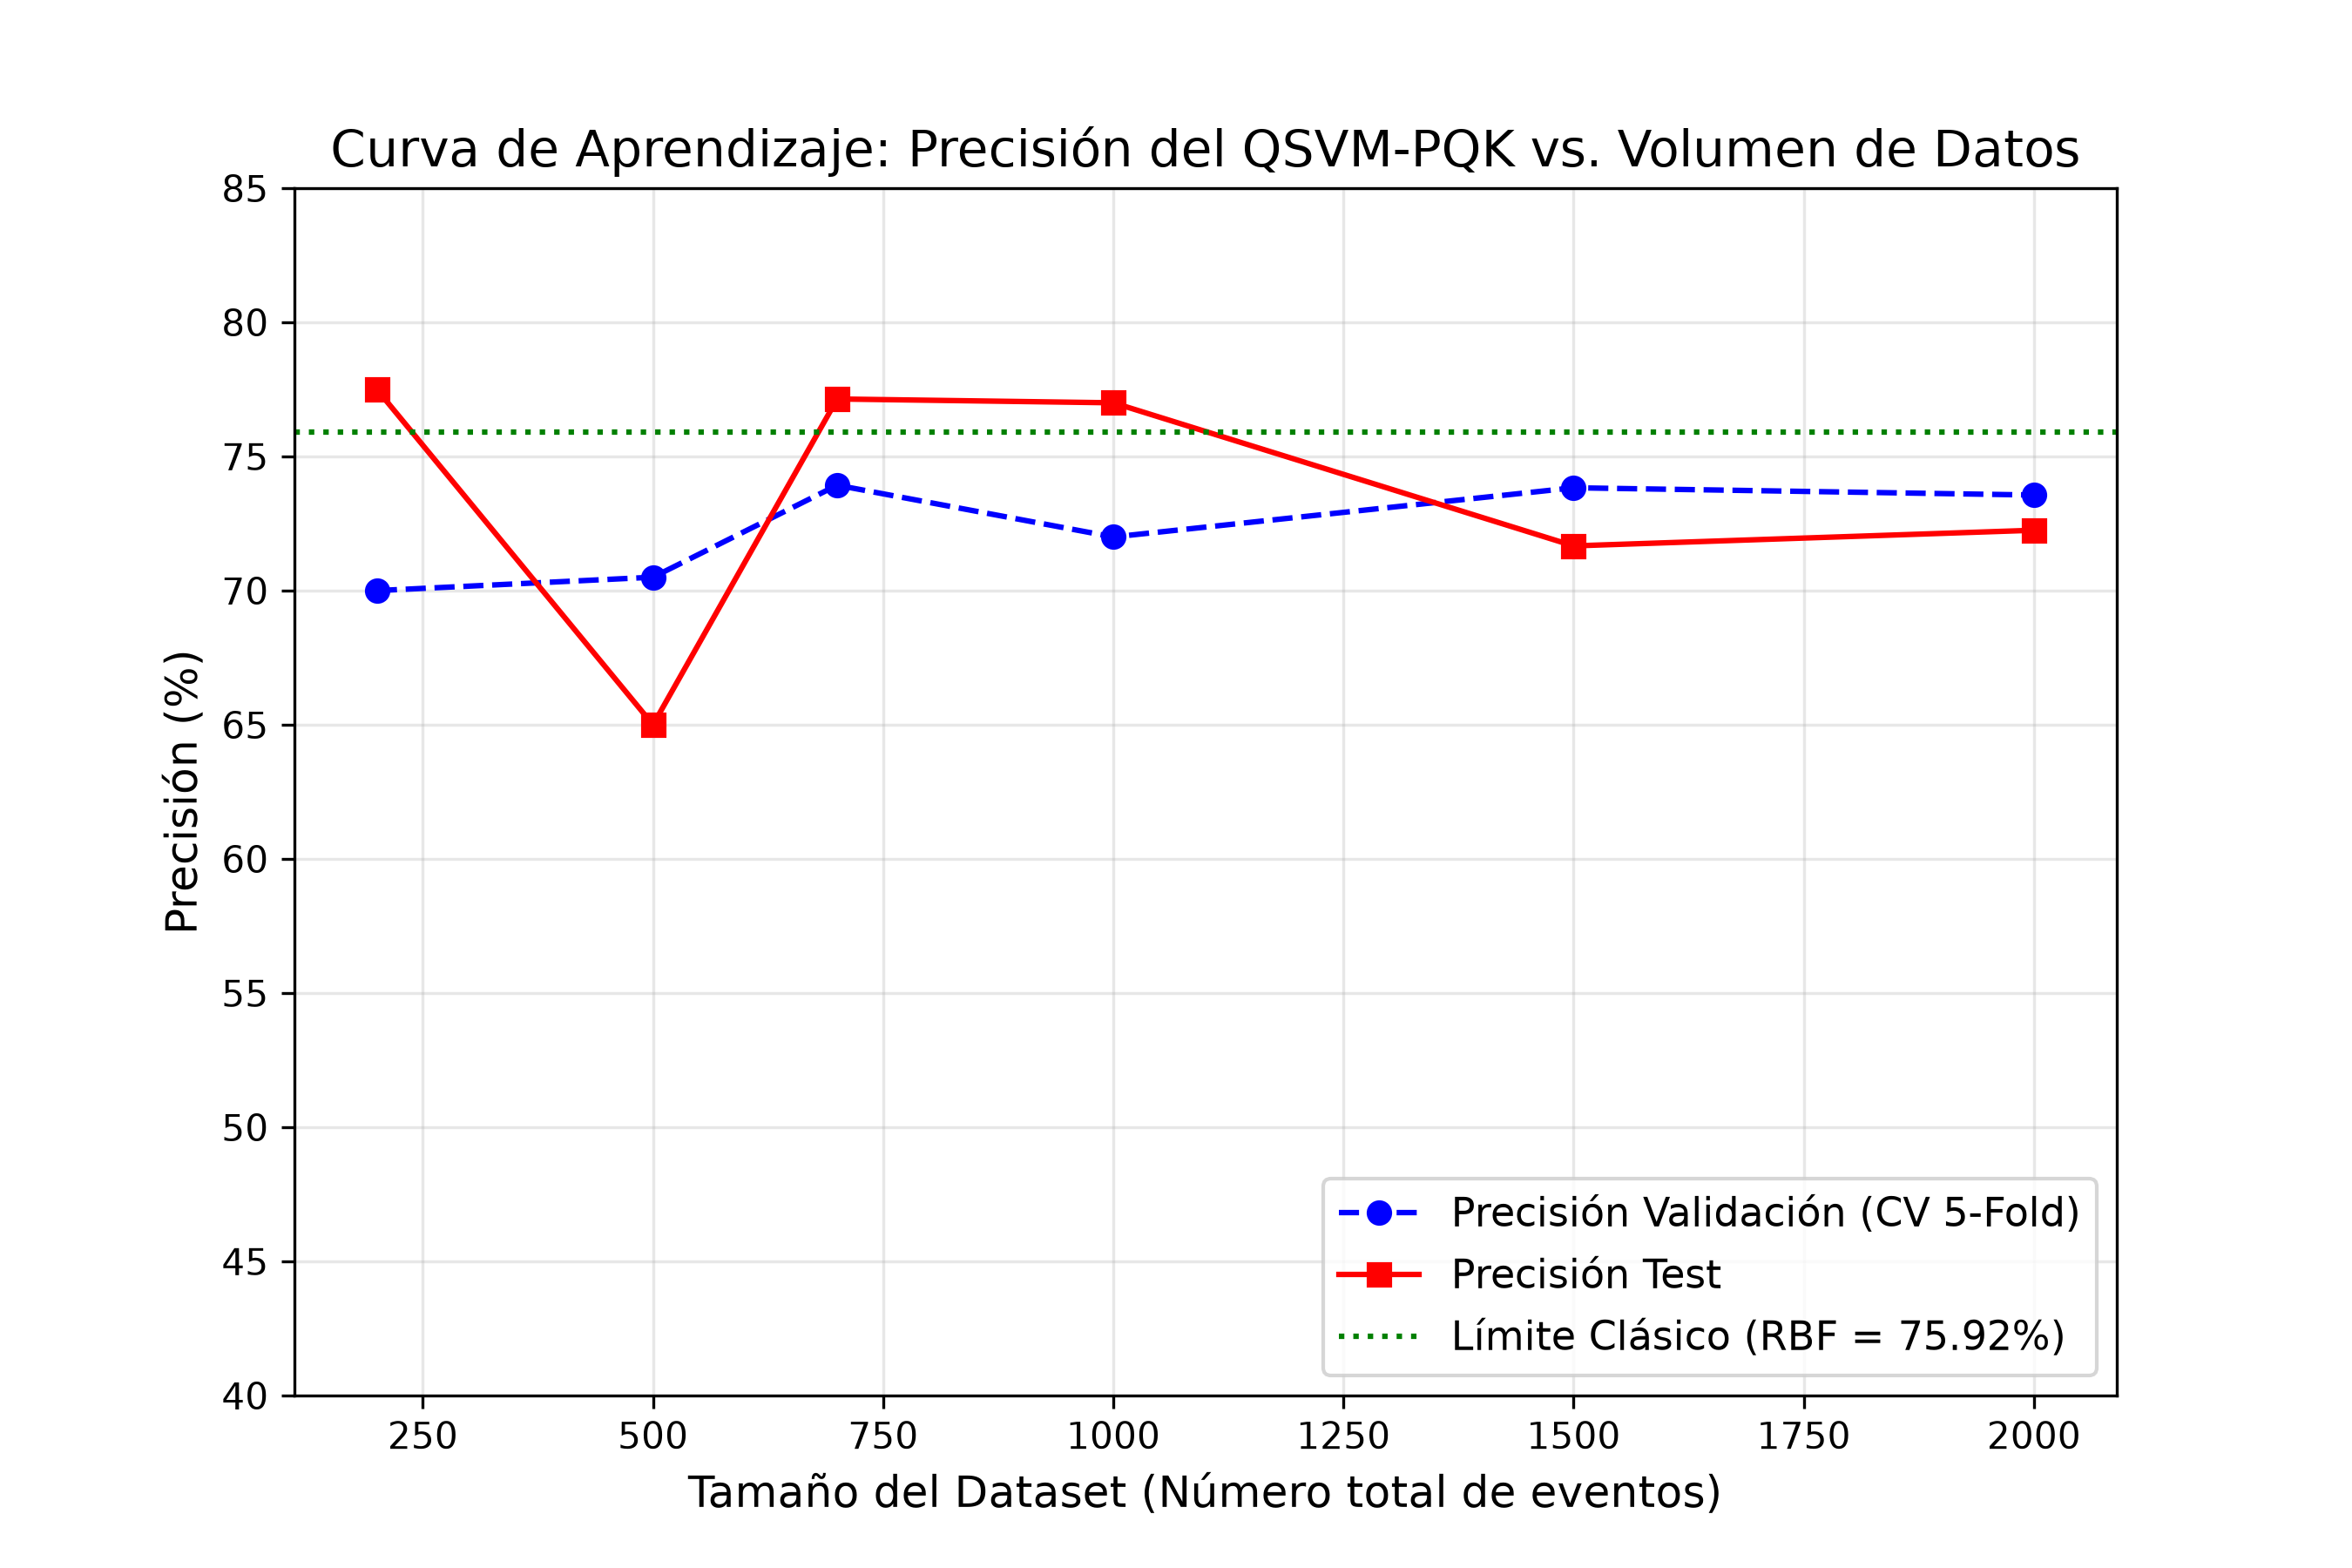
\includegraphics[width=0.7\textwidth]{curva_aprendizaje_pqk.png}
    \caption{Curva de Aprendizaje comparando precisión de validación frente al límite clásico.}
    \label{fig:curva_aprendizaje}
\end{figure}

Los resultados muestran que el rendimiento del QSVM se estabiliza asintóticamente alrededor del $73.5\%$, manteniéndose consistentemente por debajo de la cota superior del modelo RBF clásico ($75.92\%$). Adicionalmente, incrementar la profundidad del circuito a $reps=2$ redujo la precisión de validación, evidenciando saturación arquitectónica.

% ==========================================
% 4. CONCLUSIONES
% ==========================================
\section{Conclusiones y Trabajo Futuro}
El presente análisis exhaustivo demuestra que los modelos QSVM basados en \textit{ansätze} de características fijos enfrentan un límite estructural intrínseco. Aunque la proyección de observables (PQK) ofrece mejoras geométricas críticas sobre el kernel estándar (FQK), la topología rígida del circuito es incapaz de modelar la no linealidad de la cinemática pura de altas energías. 

Por consiguiente, se requiere un cambio de paradigma hacia el diseño dinámico de circuitos. Como trabajo futuro, la siguiente fase de esta investigación implementará un Algoritmo Genético (GA) bajo un esquema multiobjetivo, enfocado en evolucionar la topología del circuito cuántico (maximizando la precisión y minimizando la profundidad) para adaptarse naturalmente a las propiedades físicas del conjunto de datos SUSY y garantizar resiliencia frente al hardware cuántico de la era NISQ.

% ==========================================
% REFERENCIAS
% ==========================================
\renewcommand{\refname}{\normalsize Referencias}
\begin{thebibliography}{5}
    \footnotesize
    \bibitem{nguyen2026} 
    M. D. Nguyen, T. H. Vu, B. H. Le, y L. N. Tran. 
    \textit{Flexible genetic algorithm for quantum support vector machines}. 
    Machine Learning: Science and Technology, vol. 7, 045030, 2026.
    
    \bibitem{baldi2014}
    P. Baldi, P. Sadowski, y D. Whiteson.
    \textit{Searching for exotic particles in high-energy physics with deep learning}.
    Nature Communications, vol. 5, 4308, 2014.
    
    \bibitem{havlicek2019}
    V. Havlíček et al.
    \textit{Supervised learning with quantum-enhanced feature spaces}.
    Nature, vol. 567, pp. 209-212, 2019.
    
    \bibitem{huang2021}
    H.-Y. Huang et al.
    \textit{Power of data in quantum machine learning}.
    Nature Communications, vol. 12, 2631, 2021.
    
    \bibitem{cortes1995}
    C. Cortes y V. Vapnik.
    \textit{Support-vector networks}.
    Machine Learning, vol. 20, pp. 273-297, 1995.
\end{thebibliography}

\end{document}
